\documentclass{sigchi}

% Remove or comment out these two lines for final version
\toappearbox{\Large Submitted to CHI'13. \\Do not cite, do not circulate.}
\pagenumbering{arabic}% Arabic page numbers for submission.

% Use \toappear{...} to override the default ACM copyright statement (e.g. for preprints).

% Load basic packages
\usepackage{balance}  % to better equalize the last page
\usepackage{graphicx} % for EPS, load graphicx instead
\usepackage{times}    % comment if you want LaTeX's default font
\usepackage{url}      % llt: nicely formatted URLs
\usepackage{tabularx}
\usepackage{subfigure}

% llt: Define a global style for URLs, rather that the default one
\makeatletter
\def\url@leostyle{%
 \@ifundefined{selectfont}{\def\UrlFont{\sf}}{\def\UrlFont{\small\bf\ttfamily}}}
\makeatother
\urlstyle{leo}


% To make various LaTeX processors do the right thing with page size.
\def\pprw{8.5in}
\def\pprh{11in}
\special{papersize=\pprw,\pprh}
\setlength{\paperwidth}{\pprw}
\setlength{\paperheight}{\pprh}
\setlength{\pdfpagewidth}{\pprw}
\setlength{\pdfpageheight}{\pprh}

% Make sure hyperref comes last of your loaded packages,
% to give it a fighting chance of not being over-written,
% since its job is to redefine many LaTeX commands.
\usepackage[pdftex]{hyperref}
\hypersetup{
pdftitle={SIGCHI Conference Proceedings Format},
pdfauthor={LaTeX},
pdfkeywords={SIGCHI, proceedings, archival format},
bookmarksnumbered,
pdfstartview={FitH},
colorlinks,
citecolor=black,
filecolor=black,
linkcolor=black,
urlcolor=black,
breaklinks=true,
}

% create a shortcut to typeset table headings
\newcommand\tabhead[1]{\small\textbf{#1}}


% End of preamble. Here it comes the document.
\begin{document}

\title{Making Touchscreen Keyboards Adaptive to Keys, Hand Postures,  and Individuals---A Hierarchical Spatial Backoff Model Approach}

% Note that submissions are blind, so author information should be omitted
\numberofauthors{3}
\author{
 \alignauthor Ying Yin\\
   \affaddr{Massachusetts Institute of Technology}\\
   \affaddr{Address}\\
   \email{yingyin@mit.edu}\\
 \alignauthor Tom Ouyang\\
   \affaddr{Google}\\
   \affaddr{Address}\\
   \email{e-mail address}\\
 \alignauthor Kurt\\
   \affaddr{Affiliation}\\
   \affaddr{Address}\\
   \email{e-mail address}\\
}

% Teaser figure can go here
%\teaser{
%  \centering
%  \includegraphics{Figure1}
%  \caption{Teaser Image}
%  \label{fig:teaser}
%}

\maketitle

\begin{abstract}
The text entry prediction for touchscreen keyboards on mobile devices can be improved by adapting the underlying spatial model to factors such as input hand postures, individuals, and target key positions. To
combine these factors together, we introduce a hierarchical spatial backoff
model (SBM) that consists of submodels with different levels of
complexity. The most general model includes no adaptive factors, whereas the most specific model includes all three. Considering that in practice people may
switch hand postures (e.g., from two-thumb to one-finger) to better suit a situation,
and that the specific submodels may take time to train for each user,  a specific
submodel should be applied only if its corresponding input posture can be identified with
confidence, and if the submodel has enough training data from the user.  We
introduce the \textit{backoff} mechanism to fall back to a simpler model if
either of these conditions are not met.  We implemented a prototype system capable of reducing the language-model-independent error rate by 13.2\% using an online posture classifier with 86.4% accuracy.  Further improvements in error rate may be possible with even better posture classification.

\end{abstract}

\keywords{
 Touchscreen text input; posture adaptation; personalization; adaptive model.
}

\category{H.5.2.}{Information interfaces and presentation}{User interfaces---\textit{input devices and strategies}}

\section{Introduction}
The rapid growth of touchscreen based smartphones and tablets have made finger typing on touchscreens an everyday information input activity. Touchscreen keyboards, which can also be called Smart Touch Keyboards (STK’s), have advanced significantly in the past few years. Taking the open source Android keyboard as an example, a modern touch screen keyboard uses language modelling, spatial and edit distance based corrections, and other sophisticated techniques to predict, correct, and complete the user’s imprecise typing. Despite these engineering achievements, text input continues to be a mobile user experience bottleneck, particularly for business and productive use~\cite{Bao:2011}. Any further improvement to the mobile typing experience, even by a small amount, is desired and important since hundreds of millions of people use a smartphone or tablet everyday.

One compelling direction of research is better adaptation and personalization of keyboard spatial models. A spatial model converts each touch point into a probability distribution over the different letters on the keyboard. With soft keyboards, the underlying ``keys'' can shift and adapt to the user. Azenkot and Zhai~\cite{Azenkot:2012} did a systematic study of smartphone keyboard touch patterns under various typing conditions. We note the following observations from their study:

\begin{enumerate}
\item People use different ``hand postures''---one index finger, one thumb, and two thumbs---to type on smartphones. Depending on the situation (e.g.\ sitting, standing or walking), the same individual may also change from one hand posture to another. For example, the same individual who normally types with two thumbs on a phone while sitting down may switch to one index finger or one thumb typing while standing or walking. We cannot assume that the same individual will use the same hand posture all the time. Adaptation methods based on lab experiments with one consistent hand  posture, such as those in~\cite{Findlater:2012}, give important insights and guidance for designing practical systems. But they may also face challenges as practical solutions because user may change their hand posture in real world settings from their usual preference.

\item These hand postures change the touch typing patterns. For example, for right handed users adopting one index finger and one thumb typing postures, touches on the left side of a smartphone touchscreen keyboard tend to be biased rightward. However these touches tend to be biased leftward among users adopting two thumb postures.

\item Touch patterns can also depend on letter keys. For example, for one-finger typing, touch points tend to shift downward on the bottom letter row of a touchscreen keyboard, but not the top row (Q - P).

\item Users’ touch points tend to spread wider on a collective basis (polling all users data together) than on an individual basis for the same posture. This shows that different users tend to have different touch point distributions, but within the same user, the touch point pattern using the same posture may be more consistent.
\end{enumerate}

Together these findings make a strong case for personalization of smartphone touch keyboard algorithms. However they also illustrate the challenges and complexities of personalization. An advanced keyboard that adapts to user differences needs to account for multiple \textit{adaptive factors} in order to work effectively. For example, a personalized typing model would have limited effectiveness if it could not also adapt to hand posture. This is because the same user can have a very different typing pattern depending on whether she is typing with one finger or two. Effective adaptation may require a combinatorial approach that is key, posture, and user specific.

A combinatorial approach raises challenging implementation issues. First, there need to be a large number (e.g., 26 keys $\times$ 3 postures = 78) of submodels for each user. Collecting a sufficient amount of data to build each submodel may take too long to be practically useful, especially for infrequent letters such as, in English, ``Z'' and ``X.'' Second, if an STK does have a large number of (sub)models, model selection can be a significant challenge.  Since each submodel is specific to a combination of factors, a wrong selection may actually hurt the keyboard’s quality. Correct model selection requires an accurate identification of the current \textit{mode}, i.e.\ a combination of adaptive factors. While it is relatively easy to identify the individual (for example, by device login), it is not so easy to identify what hand posture the user is applying to each tap.

To address these challenges, we propose and explore a hierarchical backoff approach to building adaptive STK spatial models. The models in the hierarchy range from generic (e.g.\ a base model that is user, key, and posture invariant) to specific (e.g., a model that has specialized parameters for each user, key, and posture combination). When a user first starts typing on a hierarchical adaptive keyboard, it initially defaults to the base model, and the other more specific models are dormant. The system continues to collect touch points data from the user to train submodels. A submodel becomes \textit{mature} when a sufficient amount of data is available to train it. Determining the threshold for the minimum amount of data required is an essential part of the backoff model, which we discuss later in the paper.
A \textit{mature} model will continue to renew itself with new user data to accommodate  both short and long-term adaptation to changes in user behavior. If there is not enough data to train the model or the system is not confident enough that the model is appropriate, the system \textit{backs-off} to a more general model or the base model. This hierarchical backoff approach is a major contribution of this paper, and offers the following advantages for fast and robust adaptation in an STK:
\begin{enumerate}
\item It does combinatorial and fine grained adaptation, not only to the user as a single lumped entity, but also in combination with hand posture and key location factors. It is therefore more practical and less brittle since it does not assume one user will always use the same hand posture in all situations.

\item It is conservative. Posture adaptation is applied only if the posture detection is confident enough, and when its corresponding submodel is \textit{mature}. It is also designed to be conservative and biased towards the standard base model if either of these condition is not clearly satisfied. This minimizes the risk of over-adaptation and transitional instability when the user changes hand posture.

\item The system does not require a separate training (data collection) phase for each individual. It is more practical to launch such an adaptive system.

\item The system continually updates and renews itself, so it can accommodate
long-term changes in user behavior.
\end{enumerate}
We call keyboards built in such an approach SBM (spatial backoff model) keyboards. The SBM approach also raises many questions and challenges that will be addressed in the rest of the paper. Here we give a brief outline to these problems and their solutions.

First, while the observations made in Azenkot et al.~\cite{Azenkot:2012} are quite unambiguous
about key location, hand posture, and individual being potential adaptive
factors, they need further investigation.  We report one analysis on the
relative key detection power of various spatial models specific to the
combinatorial factors of key, hand posture, and individual in the ``Comparison of Spatial Model'' section below. The analysis is based on \textit{observed}
posture and user-intended key. With our dataset it was found that, compared to
the base model, posture- and key-specific spatial models could reduce character
error rate by about 11.5\%, and that user- and key-specific spatial models could
reduce character error rate by about 14.2\%. These reduction in error rates
represent theoretical upper bounds based on our dataset.

Second, in the ``Input Hand Posture Classification'' section, we present a detailed
SVM (support vector machine) classifier of hand postures that returns identification of
two-thumb or one-finger (including one-thumb and one-index-finger) posture from users' touch points while entering text. The recognition accuracy is 86.4\%.

Third, in the ``Evaluation of Standalone SBM'' section, we show that posture classification combined with adaptive models improves spatial model performance by reducing the character error rate by 13.2\% over a non-adaptive base model.

\section{Related Work}

There is a body of active research on using spatial models, language models, and a combination
of the two to improve text entry accuracy on an STK. For example,
Al Faraj et al.~\cite{AlFaraj:2009} and Magnien et al.~\cite{Magnien:2004} both use
visual highlight of the next possible keys to aid typing. Their predictions of the next keys are based on a language model which is independent of the improvements we propose through spatial model adaptation.

Kristensson et al.~\cite{Kristensson:2005} propose a geometric pattern matching technique to improve
stylus input accuracy. They match the geometric pattern of the touch points on a stylus keyboard against patterns formed by
the letter key center positions of legitimate words in a lexicon. Similar to our work,
they propose a gesture-based stylus input method in which users only need to stroke between the keys~\cite{Kristensson:2004}.
Their approach uses a combination of spatial and language models. However,
their spatial model is not adaptive. While our focus is on tapping input, the same adaptive spatial model approach
can be potentially applied to the gesture-based input.

Key-adaptive spatial models were explored by Goodman et al.~\cite{Goodman:2002}, who compute for stylus input separate bivariate Gaussian distributions with means and
covariance matrices per key. Zhai et al. also show that
the hit points for each key on a custom keyboard~\cite{Zhai:2000} are normally distributed, but furthermore that the centers of the distributions shift in different directions depending on the positions of
the keys~\cite{Zhai:2002}. In their relative keyboard input system, Rashid et al.~\cite{Rashid:2008} use a different bivariate Gaussian for each key. However, the error rate of their system is high because of the keyboard position is not fixed.

Building on~\cite{Goodman:2002}, Gunawardana et al.~\cite{Gunawardana:2010} use restricted bivariate Gaussian
models in their anchored key-target resizing method. Key-target resizing means dynamically
adjusting the underlying target areas of the keys based on their probabilities. The probabilities can
be a combination of spatial model and language model probabilities.
They argue that overly aggressive
key-target resizing can sometimes prevent a user from entering their desired text, and hence violate
his or her expectation about keyboard functionality. They ensure that a touch point within
the anchor area of a key is always detected as that key irrespective of the language model.

In personal adaptation for STK, Findlater and
Wobbrock~\cite{Findlater:2012} explored spatial model adaptation on large touch
surfaces, in which one can use ten fingers to do traditional desktop style touch
typing. Based on a user study of 12 participants, they find measurable
performance improvements when the keyboard touch typing model is able to adapt to a particular user.

In comparison to ten-finger typing on a large touch surface, the individual
differences in one-finger or two-thumb typing on smartphones are more subtle but
still compelling. Rudchenko et al.~\cite{Rudchenko:2011} developed a text entry
game for smartphones that provides targeting words for users to type to improve
their typing experience. As a side effect, the game generates labeled touch
point data that can be used as training data to build spatial models.
Their results, based on a user study of 6 participants, show that key-target
resizing based on a spatial model only, without personalization, gives an error reduction of 18.9\% over no key-target resizing.
When adding personalization, there is a further 2.84\% error reduction.
The results show the benefit of user adaptation in an ideal condition
in which the intended key is known. In real use, however, the intended key is unknown and can only be inferred from the current spatial
and language models. In our prototype implementation and evaluation we impose
this same real-world limitation. We build the user-adaptive spatial model by
probabilistically assigning a key to each of the user's touch points, without
relying on the hidden identity of the true intended key.

The user- and key-adaptive methods mentioned above all assume that a user's input posture
remains the same. As far as we are aware, our work is the first to investigate adaptation of dynamically changing postures.

There is also a body of applicable work on user modeling and adaptation not
directly related to touch keyboard typing. A system can be considered a
user-adaptive system if it makes
nontrivial inferences about properties of the user, and adapts its actions
to these inferred properties~\cite{Jameson:2000}. Some systems use rule-based
adaptation that may lack empirical justification, while others use
decision-theoretic methods (e.g.,~\cite{Jameson:1998}). Jameson et al.~\cite{Jameson:2000} argue that it is important to develop decision procedures for adaptation in a principled and
empirically justified way, and they present a method to do so based on a
Bayesian network model. We also use a data-driven approach for adaptation and build a relative simple user model compared to theirs. More work could be done in the
user-modeling direction to incorporate even more properties for
STK adaptation, e.g., whether the user is walking or sitting, the user's body
posture, etc.

The idea of backoff to a lower level model when a higher level more specific
model is not available is commonly used in language modelling for speech
recognition~\cite{Katz:1987, Zitouni:2007}. For example, when unseen
\textit{n}\mbox{-}gram events are encountered, the backoff class-based \textit{n}\mbox{-}gram
language model is used.  In language modeling, all variables are observed including backoffs.
However in our model some of the variables are observed, e.g.\ user, whereas some
are hidden and need to be inferred, e.g.\ posture. As a result, the backoff
conditions are more complicated in our model.

Finally, researchers have explored other ways to improve the
text input experience on touchscreen keyboards. One method is to vibrotactile feedback~\cite{Brewster:2007, Hoggan:2008}.
Another is to use alternative keyboard layouts optimized for typing speed (word per minute)
based on Fitts' law and character level digraph frequencies~\cite{Zhai:2000, MacKenzie:1999}.
These dimensions are orthogonal to the language and the spatial models, and can be potentially
combined together to further increase the input accuracy and speed.

\section{Research Methods}
We use a combination of HCI and ML (machine learning) methods to develop and evaluate the SBM.

We use a previously published smartphone typing dataset as the empirical basis for our training
and cross-validation~\cite{Azenkot:2012}. Briefly, the experiment involved 32
participants who were given random phrases to type on a ``data collector''
keyboard on an Android touchscreen phone.  The ``data collector'' keyboard was designed to collect data that reflected users' natural instincts, uninfluenced by the keyboard's actual performance.  The keyboard therefore displayed only an asterisk as a placeholder for each tap, and did not provide a backspace key.  The experiment was between-subjects, with each subject adopting a different hand posture.  For consistency, we remove the data
from the two left-handed users in our analysis.  This leaves 9 users
using one-index-finger input, 11 users using one-thumb input, and 10 users using
two-thumb input.  We also
filter out touch points that are 1.5 times the height of the key away from
the center of the target key. After this, there are 84,292 total touch points.

A basic dependent variable of the dataset and any models built from it
is ``character error rate.'' This is measured by the difference between the
character in the target phrase and character determined from the touch point via
a spatial model. Note that although this rate can be viewed as a percentage of the
total number of characters in the target phrase, it is to be interpreted cautiously. First, a 0\% error rate may never be achievable in this
particular dataset because the participants were asked to type naturally and
fast. Second, the absolute error rate maybe dataset-dependent and is not
necessarily what a user would experience in practice.  Nonetheless, the comparative error rates across conditions can be informative of the qualities
of different models.

To get a sense of the error variation among different input postures, we
calculate the mean error rates by checking whether each touch point lies within the
bounding box of the target key. The mean error rates per person using this method are
7.98\% (SD = 5.7) overall, 7.92\% (SD = 5.8) for one-index-finger, 6.59\% (SD =
3.7) for one-thumb, and 10.69\% (SD = 7.4) for two-thumb input respectively.
Since there is much less difference between the index finger posture and the single thumb posture, and because of posture classification reliability concerns, we combine the index-finger posture and the one-thumb posture into a single one-finger posture condition. Hence the posture class random variable $y$ can take values in the set $\mathcal{Y} = \{\text{one-finger}, \text{two-thumb}\}$.
For all evaluations below, the ratio of the number of users using one-finger input to
that using two-thumb input is kept the same for the training and testing datasets.

\section{Hierarchical Spatial Backoff Models (SBM)}
The hierarchical adaptive SBM consists a number of submodels in different
``levels'' (Figure~\ref{fig:hierarchy}). Each submodel is represented by a
bivariate Gaussian distribution~\cite{Azenkot:2012,
Goodman:2002, Rashid:2008}.
The lowest level is the base model which is key-, user-, and posture-
independent, i.e.\ all the keys have the same Gaussian
distribution $N(\underline\mu, \Lambda)$ where $\underline\mu \in \mathbb{R}^2$ is the mean
$(x, y)$ offsets from the center of each key's bounding box, and $\Lambda$ is
the $2\times 2$ covariance matrix. This is the most general model combining all data together. The higher level submodels adapt to a combination of
key positions, hand postures, and users. For example, the ``posture-adaptive'' model adapts to input posture only, which means there is one Gaussian model $N(\underline\mu_y, \Lambda_y)$ for each posture $y$ for \textit{all} keys. The ``posture- \& key-adaptive'' model adapts to both posture and key which means there is one Gaussian model $N(\underline\mu_{y, k}, \Lambda_{y, k})$ for each posture $y$ and key $k$ combination.  The highest level model has one Gaussian model $N(\underline\mu_{y,u,k}, \Lambda_{y,u,k})$ for each posture $y$, user $u$, and key $k$ combination.

\begin{figure}[tb]
 \centering
 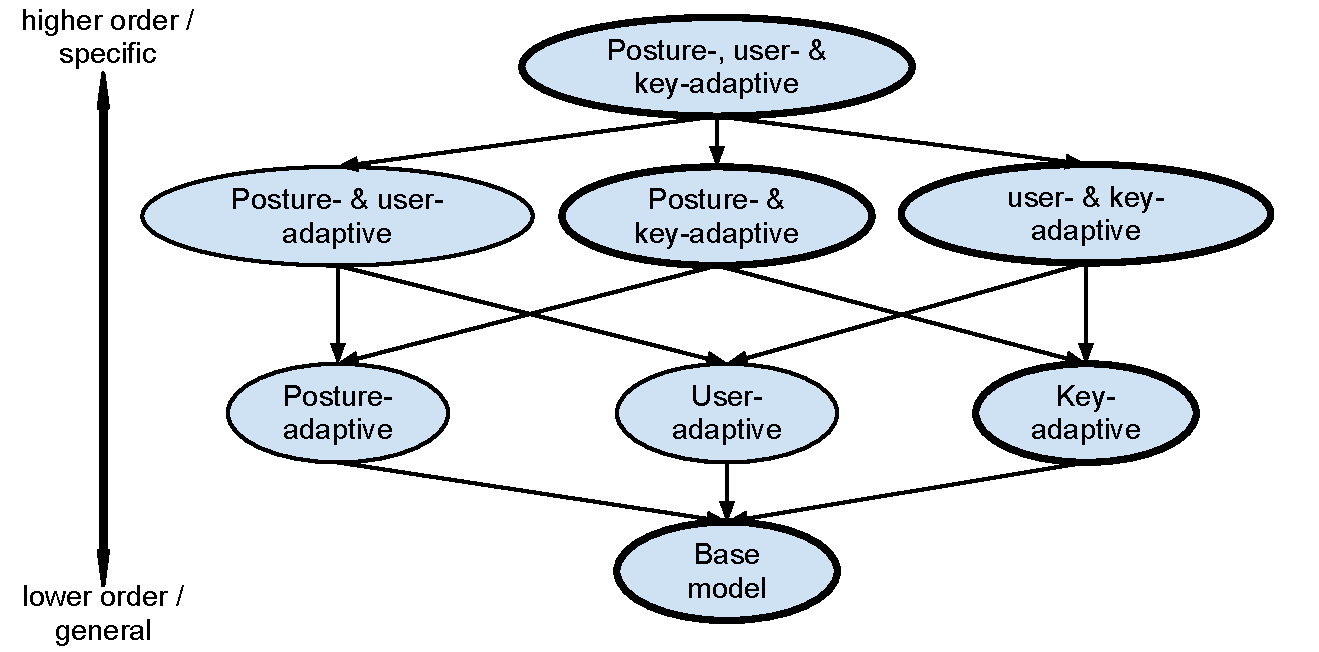
\includegraphics[width=0.9\columnwidth]{figures/hierarchy.pdf}
 \caption{A complete hierarchical spatial backoff model. For practical purposes, not all the submodels need to be included. The models with thicker lines are the ones we analyzed and included in the prototype implementation.}
 \label{fig:hierarchy}
\end{figure}

Each combination of the factors needs a sufficient number of samples to build a reliable model. Hence, each submodel would only become \textit{mature} when its reliability passes a set
threshold. Otherwise a lower order model (backoff) will be used instead.

Figure~\ref{fig:hierarchy} shows a \textit{complete} hierarchy of the submodels with all
possible combinations of the three adaptive factors. However, depending on the
relative effectiveness of the submodels, it may not be necessary to include all of
them in an implementation. In this paper, we focus on analyzing the key-adaptive model, posture- and key-adaptive model and user- and key-adaptive model.
The order of the backoff process, and the priority of the models at the same level to use can
also be design choices, but the analysis in the next section gives
guidance and suggestions on how to determine an order.

\section{Key Estimation Formulation}\label{sec:formulation}
As mentioned in the Research Methods section, our basic measure for analysis and comparison of the spatial models is character error rate. This is computed as:
\begin{align}
\text{character error rate} = \frac{\text{# wrongly estimated characters}}{\text{# all target characters}}
\end{align}

Character estimation is made based on an underlying model, which can consist of
both a language model and a spatial model.
We use $\underline\theta$ to denote the parameter vector of the overall model. Given
$i$\textsuperscript{th} touch point coordinates $\underline c_i \in \mathbb{R}^2$, we estimate the input character as the most likely intended key, $\hat k_i$,  given by the following formulation:
\begin{align}
\hat k_i &= \arg\max_k p(k | \underline c_i; \underline \theta) \\
         &= \arg\max_k \frac{p(\underline c_i, k; \underline \theta)}{\sum_k p(\underline c_i, k; \underline \theta)} \\
         &= \arg\max_k p(\underline c_i, k; \underline \theta) \\
         &= \arg\max_k p(k;\underline\theta_l)p(\underline c_i | k; \underline \theta_s) \label{eq:likely-k}
\end{align}
where $\underline\theta_l$ represents the parameter vector of the language model and $\underline\theta_s$ represents the parameter vector of the spatial model. The $p(k;\underline\theta_l)$ term is related to the frequencies of letters and is part of the language model. To investigate whether spatial model adaptation can be beneficial, we analyze key estimation using the spatial model alone as a first step. Hence we assume $p(k; \underline\theta_l)$ is the same for all $k$ (i.e.\ a uniform language model). As a result
\begin{align}
\hat k_i = \arg\max_k p(\underline c_i | k; \underline \theta_s)
\end{align}

The spatial model parameter vector $\underline \theta_s$ depends on the submodel
selected from the hierarchical SBM. For example, when the posture-, user- and key-adaptive model is selected, then
\begin{align}          
\hat k_i = \arg\max_k \sum_{y, u} N(\underline c_i - \underline o_k; \underline\mu_{y,u,k}, \Lambda_{y,u,k})[[y = \textsf{y} \wedge u = \textsf{u}]]
\end{align}
where $\underline o_k$ is the center of the visual bounding box of key $k$, and $\underline c_i - \underline o_k$
represents the offset. $\textsf{y}$ and $\textsf{u}$ represent a particular value for the posture
and the user respectively. $[[y = \textsf{y} \wedge u = \textsf{u}]] = 1$ if the
statement is true, and $0$ otherwise. Note that we use serif fonts,
e.g., $y$, to denote random variables, and use sans-serif fonts, e.g.,
$\textsf{y}$, to denote known quantities.

The above formulation assumes the values of the posture and user variables are known.  For the user variable,
this is reasonable because smartphones are personal devices and we can assume that the
same user types on the same device. For the posture variable, potentially we could
use a soft decision and combine probability distributions together based on the posture probability, $p(y)$. For the analysis in the "Comparison of Spatial Models" section below, the values for $\textsf{y}$ and $\textsf{u}$ are
\textit{observed} based on the dataset. This establishes the upper bound for the potential benefits from the adaptations. In the "Implementation and Evaluation" section, only the user is \textit{observed}; the value for the posture variable $\textsf{y}$ is \textit{inferred}.

\section{Comparison of Spatial Models}
We compare character error rate with different adaptive spatial models to analyze their
relative effectiveness (Table~\ref{tab:comparison }and Figure
\ref{fig:error-bar1})). This can suggest the order of the
backoff models to use when there is not enough data for higher level models.
10-fold cross-validation is used, and the training and testing data sets have different users.

\begin{table} [tb]
 \centering
 \begin{tabular}{|l|c|}
   \hline
   \tabhead{Spatial model} &
   \multicolumn{1}{|p{0.2\columnwidth}|}{\centering\tabhead{Character
   error rate (SD)}} \\
   \hline
   Distance from the center of the keys & 7.98\% (5.7) \\
   \hline
   \multicolumn{1}{|p{0.7\columnwidth}|}{Base model (same Gaussian model $N(\underline 0, \Lambda)$ for
   all the keys with a full covariance matrix)} & 7.85\% (5.4) \\
   \hline
   \multicolumn{1}{|p{0.7\columnwidth}|}{Key-adaptive model, $N(\underline
   \mu_k, \Lambda_k)$} & 8.02\% (5.6) \\
   \hline
   \multicolumn{1}{|p{0.7\columnwidth}|}{Posture \& key-adaptive model,
   $N(\underline \mu_{y,k}, \Lambda_{y,k})$} & 7.06\% (4.4) \\
   \hline
    \multicolumn{1}{|p{0.7\columnwidth}|}{Individual \& key-adaptive model,
    $N(\underline \mu_{u,k}, \Lambda_{u,k})$} & 6.85\% (4.4) \\
   \hline
 \end{tabular}
 \caption{Comparison of character error rate (no language model) with
 different spatial models using 10-fold cross-validation. These results represent the theoretical upper bounds for the different adaptive spatial models based on our dataset since they assume \textit{observed} postures and intended keys for building the user specific models.}
 \label{tab:comparison}
\end{table}

\begin{figure}[tb]
 \centering
 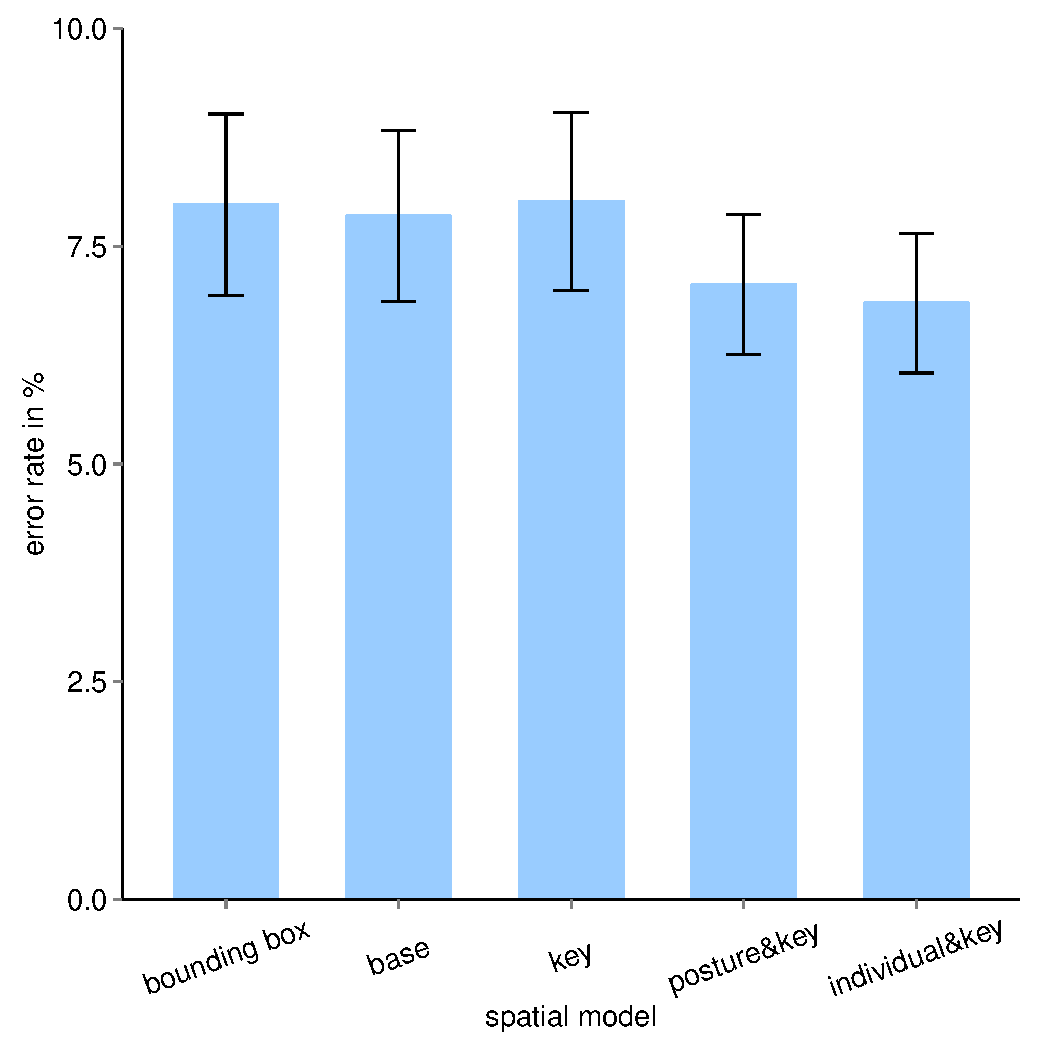
\includegraphics[width=0.8\columnwidth,
 height=0.6\columnwidth]{figures/error-rates.pdf}
 \caption{Bar plot of error rates in Table \ref{tab:comparison} with error bars
 indicating the standard error of the mean (SEM).}
 \label{fig:error-bar1}
\end{figure}

The simplest model is a Gaussian distribution with zero mean and the same spherical covariance matrix for all the keys. This model detects keys by choosing the key with the shortest Euclidean distance from the tapping coordinates.
Our base model has a full covariance matrix $\Lambda$ trained from the
training data, but the same base model $N(\underline 0, \Lambda)$ is used for all keys. Hence, when using the base model for key estimation, the most likely intended key is
\begin{align}          
\hat k = \arg\max_k N(\underline c_i - \underline o_k; \underline 0, \Lambda)
\end{align}


\subsection{Key Adaptation}
A basic key-adaptive model has one bivariate Gaussian model
$N(\underline\mu_k, \Lambda_k)$ for each key $k$ built  using data from all users in the training dataset. The most likely intended key based on key-adaptive model is
\begin{align}          
\hat k_i = \arg\max_k N(\underline c_i - \underline o_k; \underline \mu_k, \Lambda_k)
\end{align}

The result in Table~\ref{tab:comparison} shows that the key-adaptive
model has a higher error rate than the base model. A little investigation shows that different hand
postures tend to shift key specific spatial model in different ways, sometimes even in opposite
directions. For example, in Figure~\ref{fig:key-adaptive}, we observe that the
effective area of the ``W'' key goes slightly beyond the visual key boundary between ``E''
and ``W.'' For one-finger input, there tend to right horizontal offsets for ``W'' key,
while for two-thumb input, there tend to be left horizontal offsets. When mixing
these opposite effects together in key adaptation, no meaningful results could
be expected. The base model suffers the same setback, but even though neither
of the two models closely models the underlying distributions of the touch points, the base model, with fewer parameters than the key-adaptive model, may be more generalizable when there are limited data.

\begin{figure}[tb]
 \centering
 \subfigure[Key-adaptive model]{
   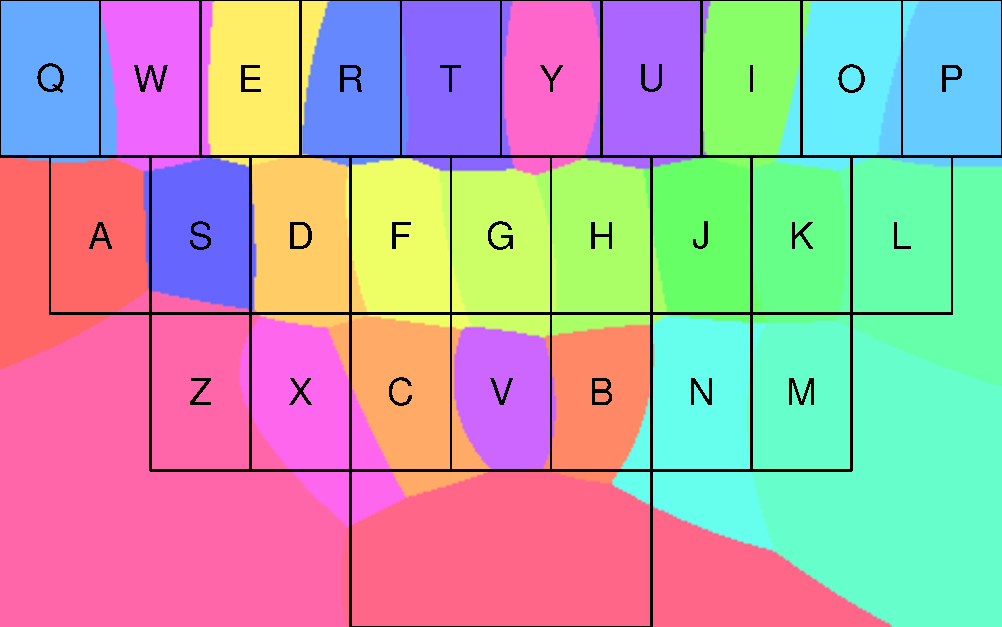
\includegraphics[width=0.47\columnwidth]{figures/key-model.pdf}
   \label{fig:key-adaptive}
 } ~
 \subfigure[Posture- and key-adaptive model for one-finger input]{
   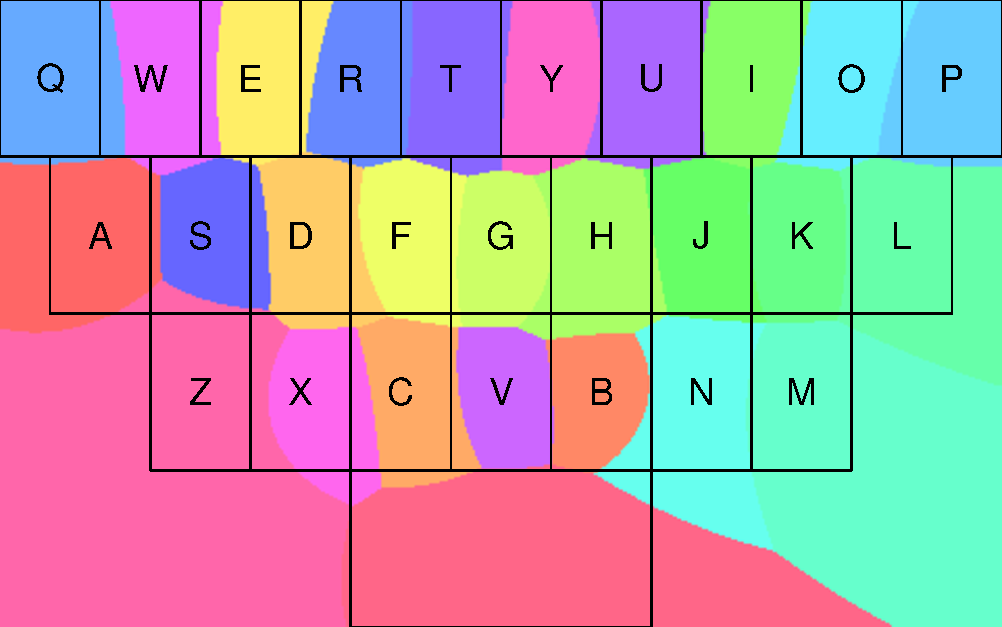
\includegraphics[width=0.47\columnwidth]{figures/posture-t.pdf}
   \label{fig:one-finger}
 }
 \subfigure[Posture- and key-adaptive model for two-thumb input]{
   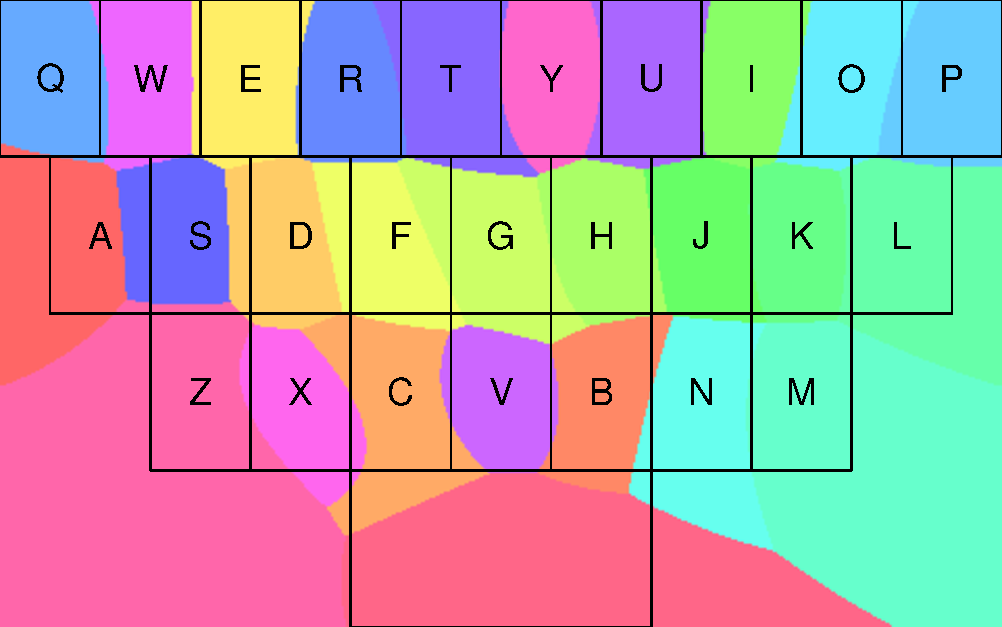
\includegraphics[width=0.47\columnwidth]{figures/posture-tt.pdf}
   \label{fig:two-thumb}
 }
 \caption{Comparison of effective key areas with different spatial models.  Each colored area presents the region such that if the user taps in that region, the spatial model will classify that key with the corresponding key label.}
 \label{fig:key-boundary}
\end{figure}

\subsection{Posture Adaptation}
Key adaptation becomes more effective when combined with posture adaptation as
shown in Table~\ref{tab:comparison}. There is 12.0\% reduction in error rate
compared to key adaptation only. A two-sample one-sided paired t-test shows
that the improvement in accuracy is significant when using posture and key
adaptation versus key adaptation only (t(29) = -2.4421, p = 0.01).

There can be different levels of complexity for posture adaptation. For the most complex one, we can have
two models for each key for each input posture, i.e., $N(\underline \mu_{y,k}, \Lambda_{y,k})$ for $y \in
\{\text{one-finger, two-thumb}\}$; or we can do posture adaptation only for a certain
number of keys, for examples for keys on the left side only or a smaller subset of keys on the left side. We experimented with these options and the best result obtained is when posture adaptation is applied to the keys on
the left side while keeping the Gaussian models for the keys on the right side independent of postures, i.e., $N(\underline\mu_k, \Lambda_k)$.
The error rate for posture and key adaption shown in Table~\ref{tab:comparison} is based on
this option. This approach is similar to the ``parameter tying'' technique that is often used in acoustic modeling in speech recognition~\cite{Bellegarda:1989} and natural language processing~\cite{Lin:1995} to deal with insufficient training data.

From (\ref{eq:likely-k}), the most likely intended key based on posture- and key-adaptive model can be written as
\begin{align}          
\hat k_i = \arg\max_k \sum_{y} p(\underline c_i | k, y; \underline\theta_s)[[y = \textsf{y}]],
\end{align}
where
\begin{align}
p(\underline c_i | k, y; \underline\theta_s) = \left\{
 \begin{array}{l l}
 N(\underline c_i - \underline o_k; \underline \mu_{y, k}, \Lambda_{y,k}) & \text{if $k$ is on left side} \\
 N(\underline c_i - \underline o_k; \underline \mu_{k}, \Lambda_{k}) & \text{if $k$ is on right side} \\
\end{array} \right.
\end{align}

The choice of this set of keys is not arbitrary. As observed by Azenkot et al.~\cite{Azenkot:2012}, the difference in horizontal
offsets of the touch points from different postures are most prominent for the keys on the
left side (Note that for left-handed users, the reverse is probably true).
In addition, the analysis of variance based on the tapping coordinates from the
dataset shows that, for different postures, there are significant differences in the means of
the $x$ coordinate for the keys on the left side of the keyboard ($p < 0.05$).

Figures~\ref{fig:one-finger} and \ref{fig:two-thumb} show the comparison of effective areas of the keys
with spatial models adapted to one-finger input and two-thumb input respectively. Note how the key areas for the left-side keys shift to the left
for two-thumb input, and shift to the right for one-finger input. The difference in
the effective key areas is the same concept as key-target resizing mentioned in~\cite{Gunawardana:2010, Rudchenko:2011}.

The error rate in Table~\ref{tab:comparison} is based on perfect knowledge of
the posture. In a deployed system, the online posture classification may
introduce errors. To mitigate the problem, the posture-adaptive model can be enabled only
if the posture classification confidence is high. The details are explained in ``Evaluation of Standalone SBM’’ section.

\subsection{User Adaptation}
The user- and key-adaptive model reduces the error rate by 14.7\% over the key-adaptive model. As some data is needed to build the user and key-specific model, the most likely intended key $\hat k_i$ can be written as:
\begin{align}          
\hat k_i = \arg\max_k \sum_{u} p(\underline c_i | k, u; \underline\theta_s)[[u = \textsf{u}]],
\end{align}
where
\begin{align}
p(\underline c_i | k, u; \underline\theta_s) = \left\{
 \begin{array}{l l}
 N(\underline c_i - \underline o_k; \underline \mu_{k}, \Lambda_{k}) & \text{if $i \le T_\text{user}$} \\
 N(\underline c_i -  \underline o_k; \underline \mu_{u, k}, \Lambda_{u, k}) & \text{if $i >T_\text{user}$} \\
\end{array} \right. \label{eq:user-adaptive}
\end{align}
$T_\text{user}$ is the minimum number of data points needed to build a user-specific key model. Equation~(\ref{eq:user-adaptive})
shows the backoff mechanism for the user- and key-adaptive model. The threshold can also be key dependent, i.e.\ $T_\text{user, k}$ for each key $k$. We have not experimented with this variation and this can be part of the future work.

The result in the last row of Table~\ref{tab:comparison} is computed by the
following method. For each fold of the cross-validation, data from the training set are used to
train the combined backoff key models. For each user $u$ in the test set,
50\% of the data for each key is used to train the user- and key-adaptive
model, i.e., $N(\underline \mu_{u, k}, \Lambda_{u, k})$.
The intended keys of these data points are evaluated on the combined backoff key models.
The remaining 50\% of the test data for each user are evaluated on the user- and key-adaptive
model.

The black line in Figure~\ref{fig:user-adapt} shows how key estimation error rate for the ``E'' key
changes as the number of points used to build
the personalized model for key E increases. The green line indicates the error rate when using the key-adaptive model only. The error rates are obtained using cross-validation
and are based on the touch points that are not used in building the
model. We choose E as an
example because it has the most number of data points (around 90) for each
user in our dataset besides the ``Space'' key. It is hard to do the analysis for the other keys with
relatively small number of data points. However, we believe the result would be applicable to other
keys. Also due to the limited number
of data points, we only show the trend until the number of touch points used to build the user
model is 70. Nevertheless, the figure still shows a general trend, and suggests
that the minimum number of data points for building a user- and key-adaptive model
should be at least 55 when the error rate becomes lower than that when using key-adaptive model alone. This is only a single data point for one key, but since it's cross-validated and averaged over several users, it is probably not too far from the real threshold.

\begin{figure}[tb]
 \centering
 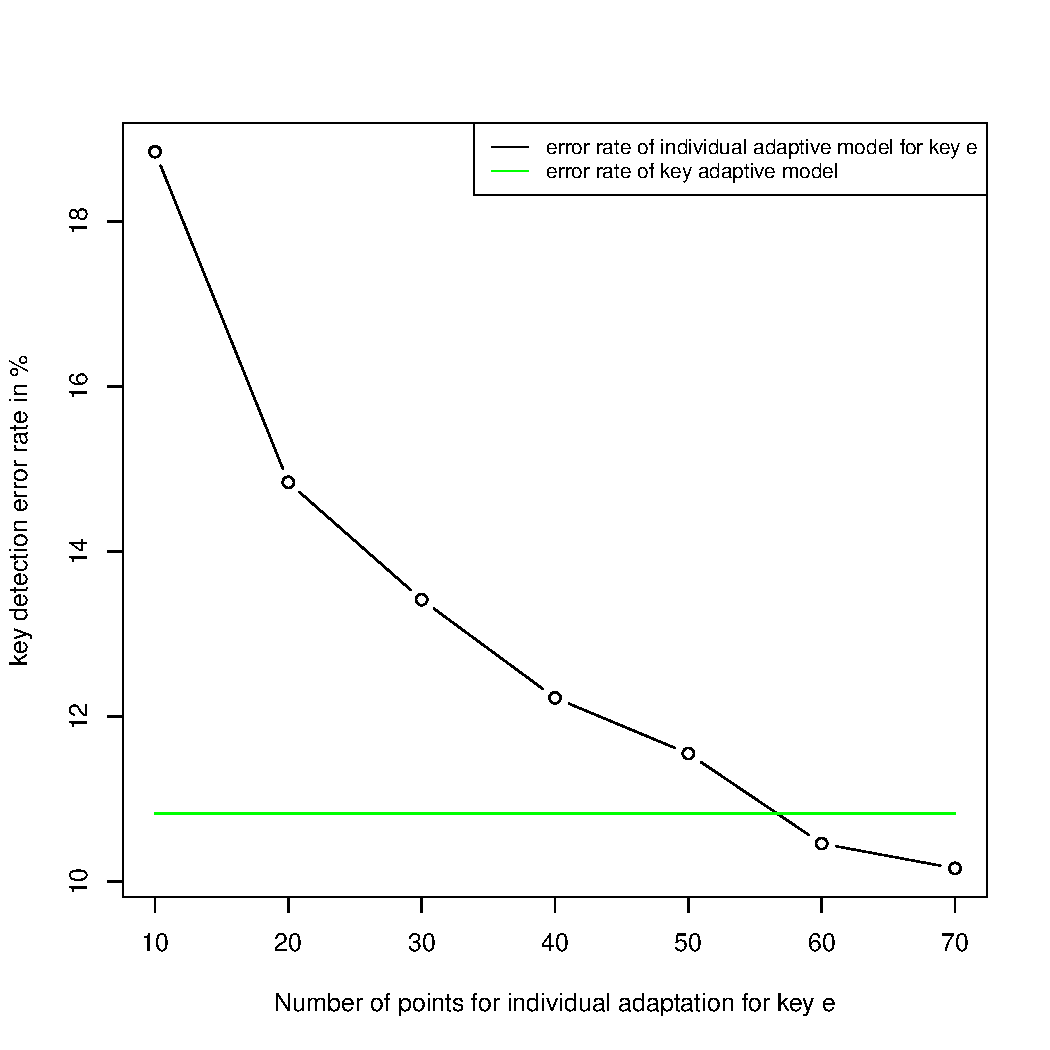
\includegraphics[width=0.9\columnwidth]{figures/individual-adapt.pdf}
 \caption{Graph showing how key estimation error rate for key E changes as the number of
 points used to build the user-adaptive model for key E increases.}
 \label{fig:user-adapt}
\end{figure}

\section{Input Hand Posture Classification}\label{sec:posture-classification}
The posture-adaptive model requires a real-time posture classifier.  For this paper, we have developed a classifier that continuously estimates $y \in \{\text{two-thumb, one-finger}\}$ from only the user's input touch points.  Note that a variety of sensor, signals, and algorithms could be used, but optimal posture classification is not the primary goal of this paper.

Our method is based on Fitts' law, which states that the time ($T$) required to
move to a target is a function of the distance ($D$) to the target and the size ($W$) of the target:
\begin{align}
T = a + b\log_2(1 + \frac{D}{W})
\end{align}                                                  
We expect Fitts' law to fit one-finger input posture well, but not two-thumb posture. For example, a user may take a longer time than average to type the letters ``AL'' using one
finger because the finger has to travel a long distance from the ``A'' key to the ``L'' key on
a Qwerty keyboard. But with two thumbs, typing ``AL'' can be faster than average because different hands are used for each key.  No long distance move is required.

%
% \begin{figure}[tb]
%   \centering
%   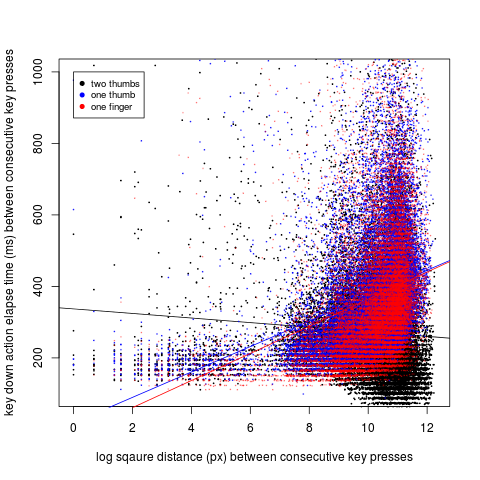
\includegraphics[width=0.9\columnwidth]{figures/time-distance.png}
%   \caption{Touch points data from input on a Nexus S phone.}
%   \label{fig:time-distance}
% \end{figure}

The analysis of the touch point data confirms this hypothesis. For the
one-finger input, the time taken increases with the distance
moved, whereas for the two-thumb input, there is no obvious trend. The
difference is more significant when the log distance (natural log)
between two consecutive touch points is greater than 5.

Based on this finding, we include the time elapsed and the log distance
between two consecutive touch points as two features for the posture classifier.
To account for individual typing speed differences, we also use normalized time
elapsed between consecutive key presses as the third feature. It is calculated
by dividing the time elapsed since the last touch point by the average time elapsed for the last 10 touch points.

Using 20 users’ data for training and 10 users’ data for testing, we train an SVM classifier offline using these three features.  Each input touch point satisfies condition $C$: it is
on the other side of the keyboard from the previous touch point, and the log distance from the previous touch point is at least 5. This classifier gives a probability score $p_y^{\text{single}}$ for these touch points. Note that $\displaystyle\sum_{y \in \mathcal{Y}}p_y^{\text{single}} = 1$. The posture classification accuracy for these touch points is 83.6\%.

In order to classify every key tap and assuming the user does not change posture
rapidly, we look at a sliding time window of 10 touch points (about 2 words). For
each time window, we use another SVM classifier with the following features:
\begin{enumerate}
\item Correlation between time elapsed and log distance (this feature has the
advantage of being speed independent)
\item Sum of $p_\text{one-finger}^{\text{single}}$ for touch points satisfying condition $C$.
\item Sum $p_\text{two-thumb}^{\text{single}}$ for touch points satisfying condition $C$.
\item Number of touch points within the window classified as one-finger input.
\item Number of touch points within the window classified as two-thumb input.
\end{enumerate}
Features 2-4 are also normalized by the window size. The history of the touch points are cleared for every new typing session.
The choice of the size of the sliding window represents a trade-off between the
accuracy of the classification and how responsive the system is when the user
changes posture. We assumed that the user does not change posture
more often than every two words.  We leave validating this assumption to future work.
% even to test with a window that does not consider history at all.

The sliding time window classifier gives a final probability score $p_y$ for posture
$y$ for each touch point. Again $\displaystyle\sum_{y\in \mathcal{Y}}p_y = 1$. To evaluate the classification accuracy, we set the the
classified posture to be $y$ if $p_y > 0.5$. With this threshold, the overall classification
accuracy for each touch point with a sliding time window
is 86.4\% (23,128 out of 26,769 touch points).

In the sliding window approach, the posture for the first few touch points  
of a new session is unknown. In this situation, a system can back off to a lower level spatial
model (key-adaptive or base model). Furthermore it can enable the posture
adaptive spatial model only when the probability score for one posture is much
higher than the other.

% \begin{figure}[tb]
%   \centering
%   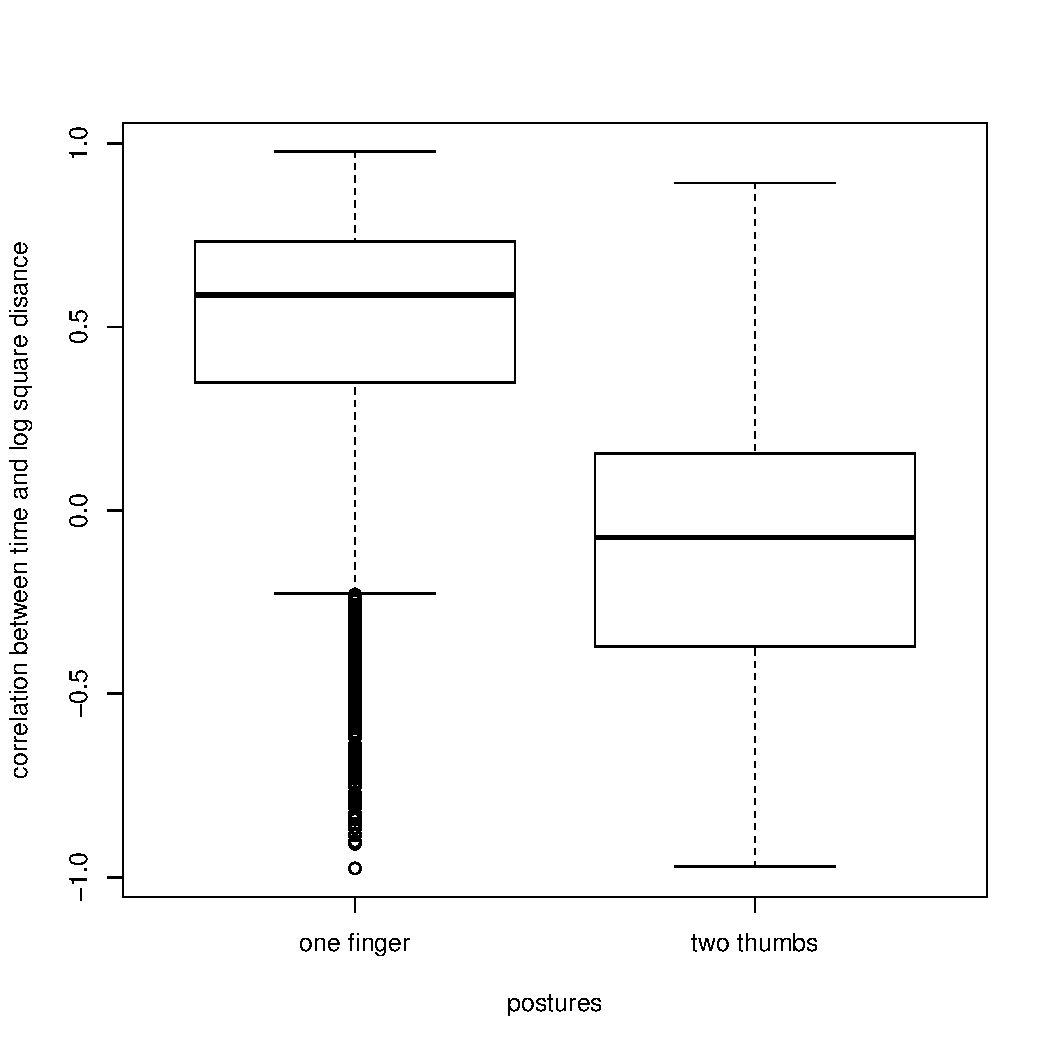
\includegraphics[width=0.8\columnwidth]{figures/boxplot.pdf}
%   \caption{Correlation between time elapsed and log square distance between
%   consecutive key presses for every 10 keys. There is a stronger correlation for
%   one- finger input than that for two-thumb input.}
%   \label{fig:boxplot}
% \end{figure}

\section{Implementation and Evaluation}
The key estimation process with the proposed SBM fits nicely with the
Chain of Responsibility design pattern. Each higher level model can
hold one or more references to lower level models. Given a touch
point, the system queries the highest level model for a Gaussian
submodel for a particular user/posture/key combination. If not present,
the higher model calls the lower model, and the
query propagates until a Gaussian submodel is found.

Based on this design, we implemented a prototype of SBM with online posture
classification in C++. The prototype has flags to turn on/off certain adaptive
models so that we can easily compare their performance.
For all the evaluations, we use 20 users' data for training both the posture classifier
and the spatial models, and the other 10 users' data for testing.

\subsection{Evaluation of Standalone SBM}
Like Findlater et al.~\cite{Findlater:2012} and Rudchenko et al.~\ciite{Rudchenko:2011}, we evaluate the effectiveness of the standalone SBM  prototype on key estimation without a language model.
Table~\ref{tab:off-device} and Figure~\ref{fig:error-bar2} show the comparison of
character error rates using SBM with different submodels turned on. The main difference between these results and those in Table~\ref{tab:comparison} is that in the prototype implementation, posture is \textit{inferred} and the user specific model is built according to \textit{inferred} intended key.

\begin{table}[tb]
 \centering
 \begin{tabular}{|l|c|}
 \hline
 \tabhead{Highest level spatial model in SBM} &  
 \multicolumn{1}{|p{0.2\columnwidth}|}{\centering\tabhead{Character error rate
 (SD)}}
 \\
 \hline
Base model & 8.64\% (5.1)\\
 \hline
 Key-adaptive model & 8.71\% (5.1) \\
 \hline
   \multicolumn{1}{|p{0.7\columnwidth}|}{Posture- and key-adaptive model} &
   8.39\% (5.0)\\
 \hline
 User- and key-adaptive model  & 7.62\% (4.8)
 \\
 \hline
 Posture-, user- and key-adaptive model &  7.50\% (4.5)
 \\
 \hline
 \end{tabular}
 \caption{Comparison of character error rates using the real-world implementation of the standalone SBM model across different submodels.  These results are based on \textit{inferred} postures and intended keys for building the user specific models. Results are based on 10 test users.}
 \label{tab:off-device}
\end{table}

\begin{figure}[tb]
 \centering
 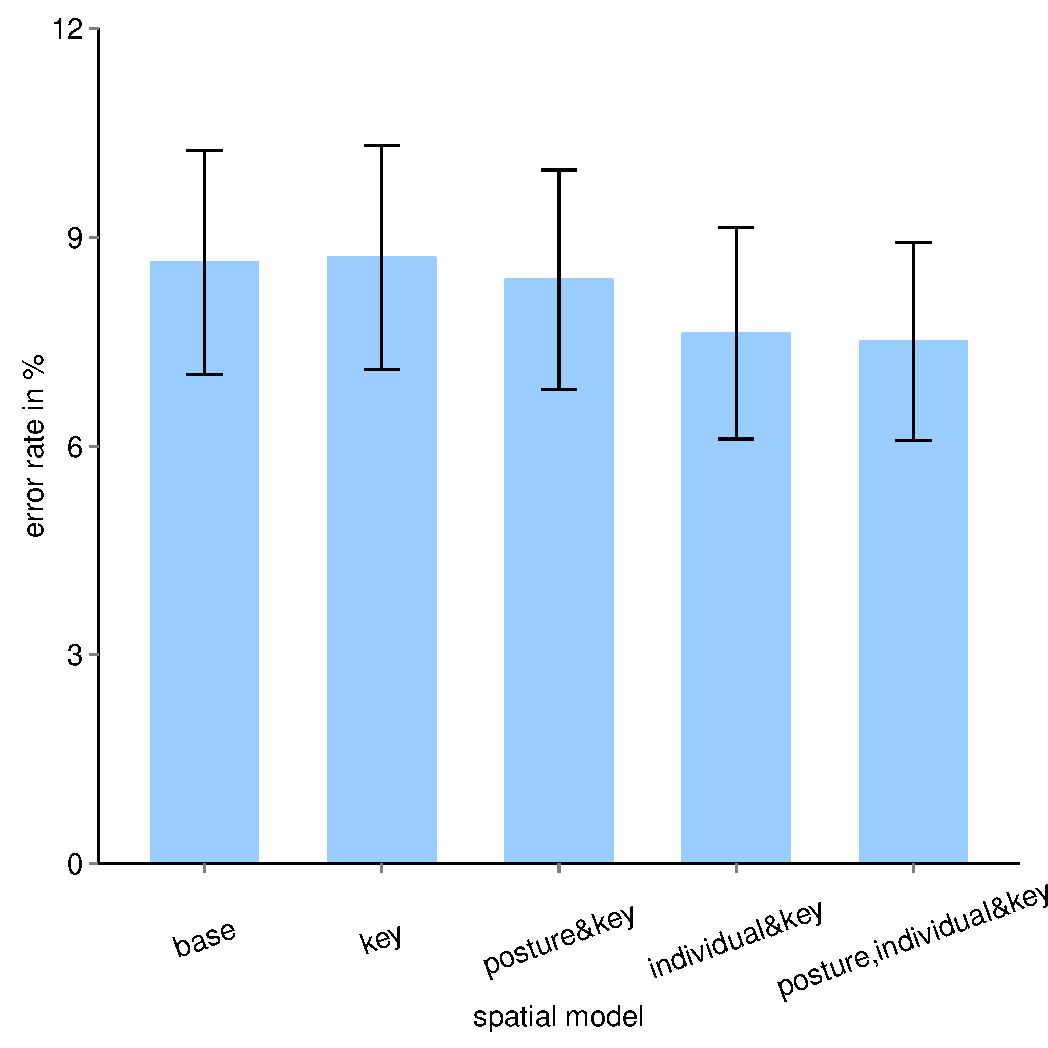
\includegraphics[width=0.8\columnwidth,
    height=0.6\columnwidth]{figures/error-rates2.pdf}
 \caption{Bar plot of error rates in Table \ref{tab:off-device} with error
 bars indicating standard error of the mean (SEM).}
 \label{fig:error-bar2}
\end{figure}

\subsubsection{Posture Adaptation}\label{sec:off-device-posture}
The posture- and key-adaptive model uses the posture classification
method described in the previous section. As a result, the
key detection error rate for this model is compounded by the posture
classification error rate.

An error in posture classification will lead to an incorrect submodel,
and hence adversely affect the key detection accuracy. To minimize incorrect classifications, we consider the confidence of the classifier.  The classifier's confidence can be determined by examining the pair of probability
scores $(p_{\text{one-finger}}, p_{\text{two-thumb}})$.
We can set a threshold $T_{\text{posture}}$ such that the input posture is classified
as $\textsf{y}$ only if $P_\textsf{y} \ge T_{\text{posture}}$. Otherwise the posture is treated as
unknown and we backoff to a lower-level spatial model.

There is a trade-off in setting the $T_{\text{posture}}$ threshold. When
$T_{\text{posture}}$ is higher, there will be fewer errors in posture classification, but also more touch points classified as unknown posture. No posture adaptation can be used for these touch points. Figure~\ref{fig:posture-confidence}
shows that there is an optimal level of the threshold beyond which the error rate
increases because we can no longer take advantage of posture adaptation. The error rate in Table~\ref{tab:off-device} for SBM with posture- and key-adaptive model as the highest order model is obtained by setting $T_{\text{posture}} = 0.94$.

\begin{figure}[tb]
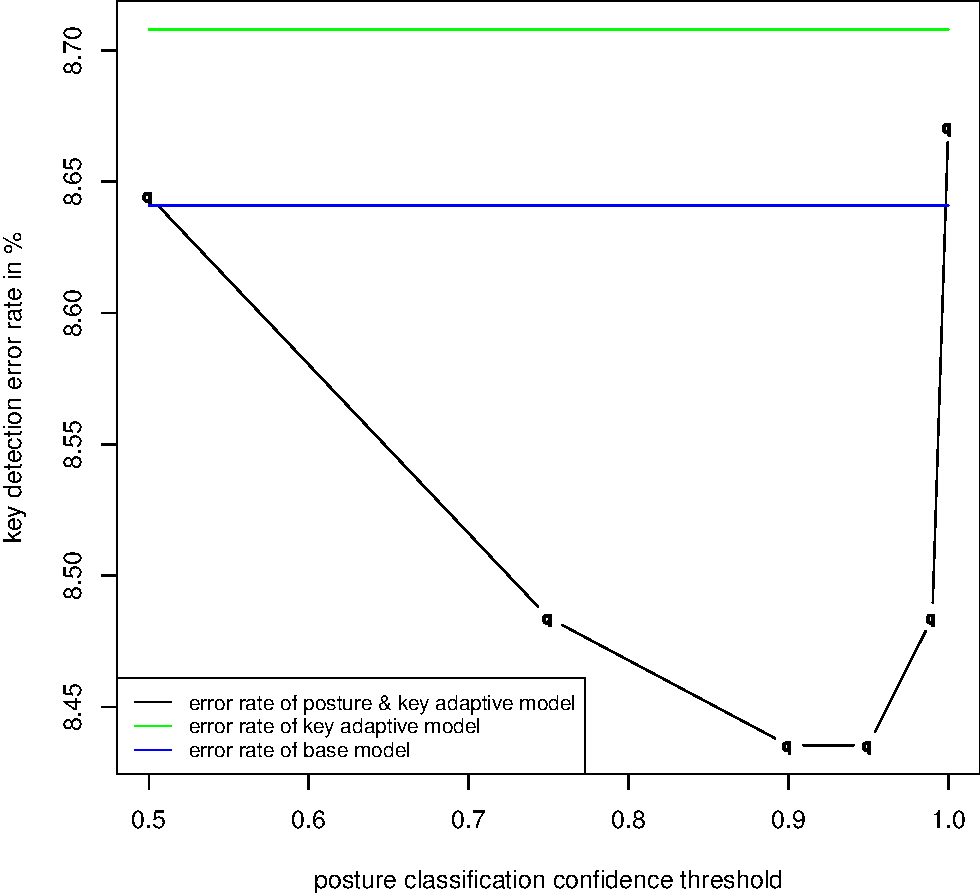
\includegraphics[width=0.9\columnwidth]{figures/error-confidence-cropped.pdf}
 \caption{Graph showing how key estimation error rate changes as the confidence
 threshold for posture classification increases.}
 \label{fig:posture-confidence}
\end{figure}

% \begin{figure*}[tb]
%   \centering
%   \subfigure[Errors when using key-adaptive model]{
%     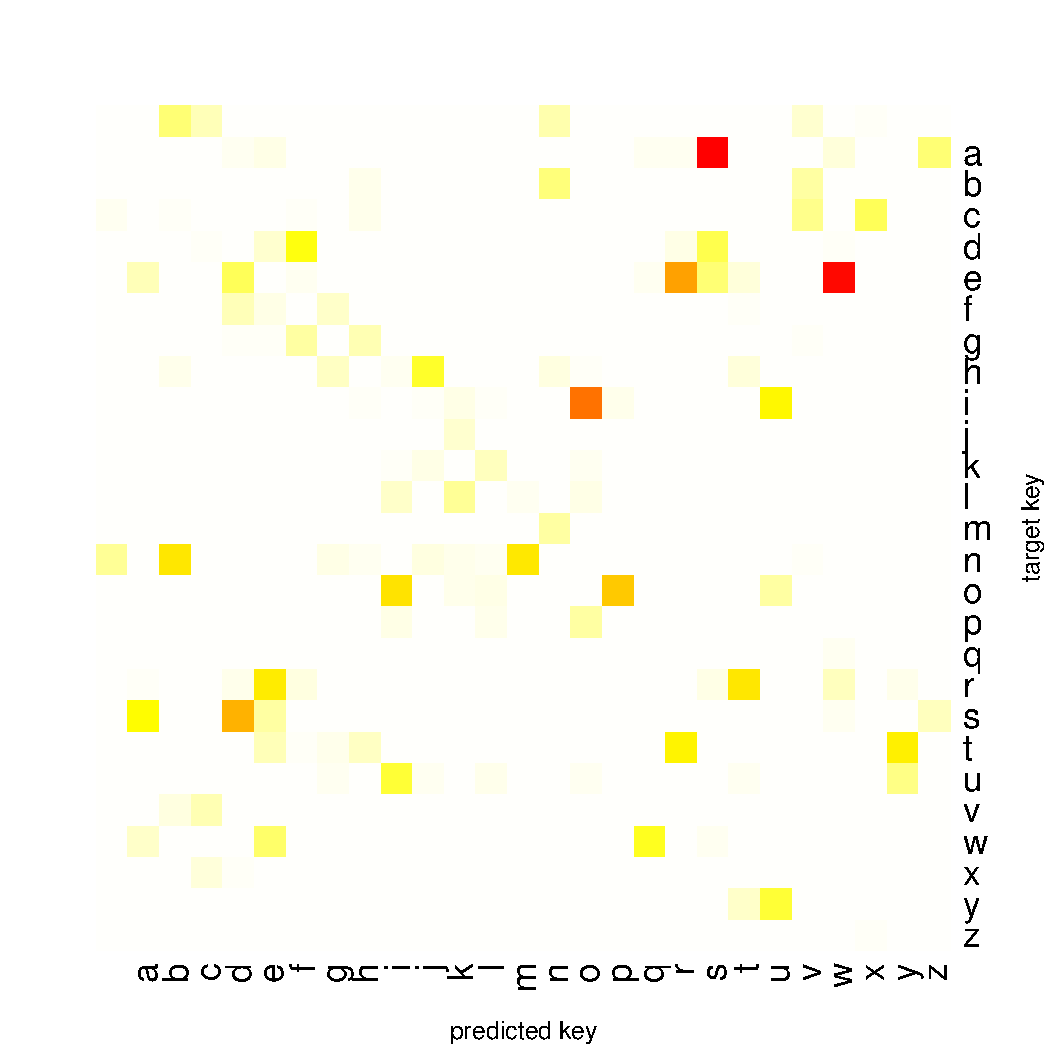
\includegraphics[width=0.49\columnwidth]{figures/sim-result-1.pdf}
%     \label{fig:error-key}
%   }
%   \subfigure[Errors when using posture- and key-adaptive model]{
%     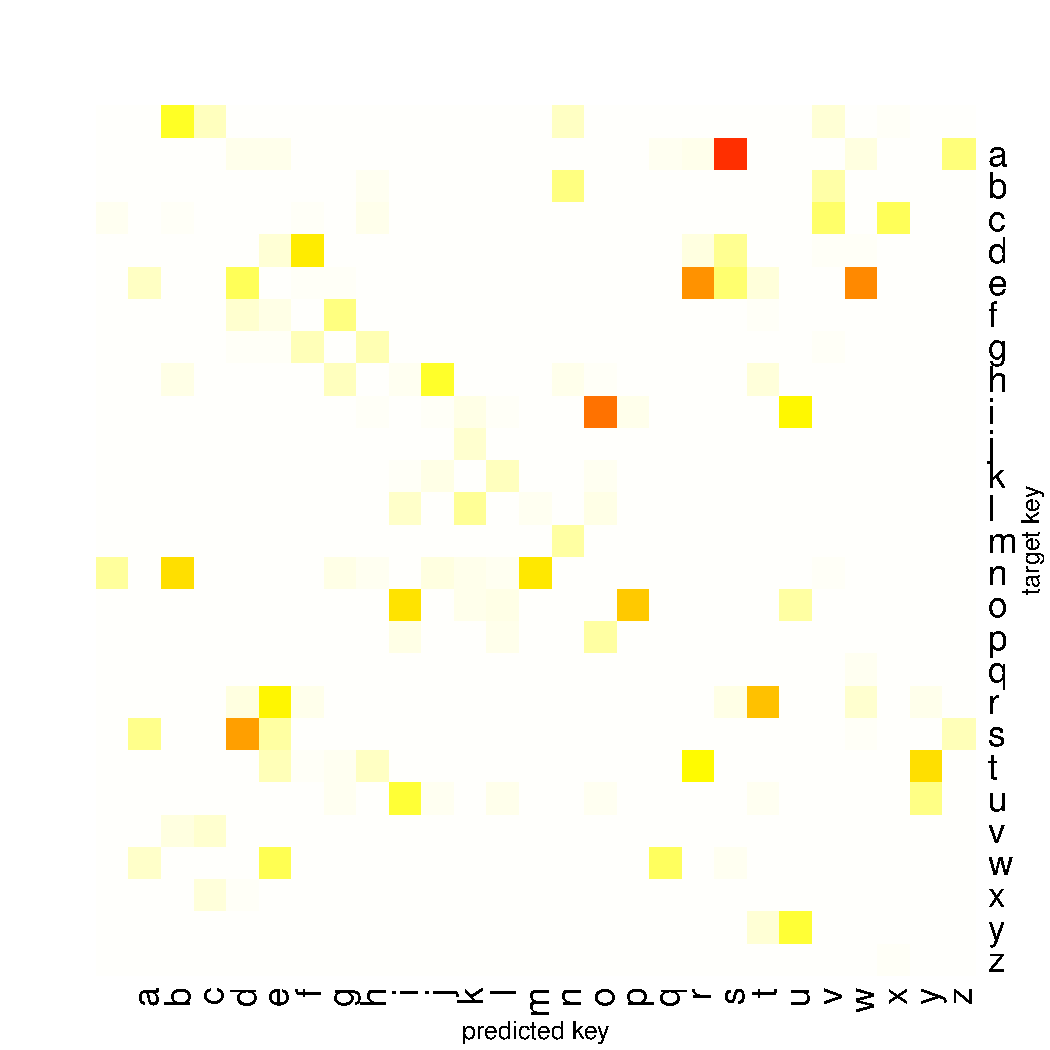
\includegraphics[width=0.49\columnwidth]{figures/sim-result-2.pdf}
%     \label{fig:error-posture}
%   }
%   \subfigure[Errors when using key-adaptive model but not when using posture- and key-
%   adaptive model]{
%     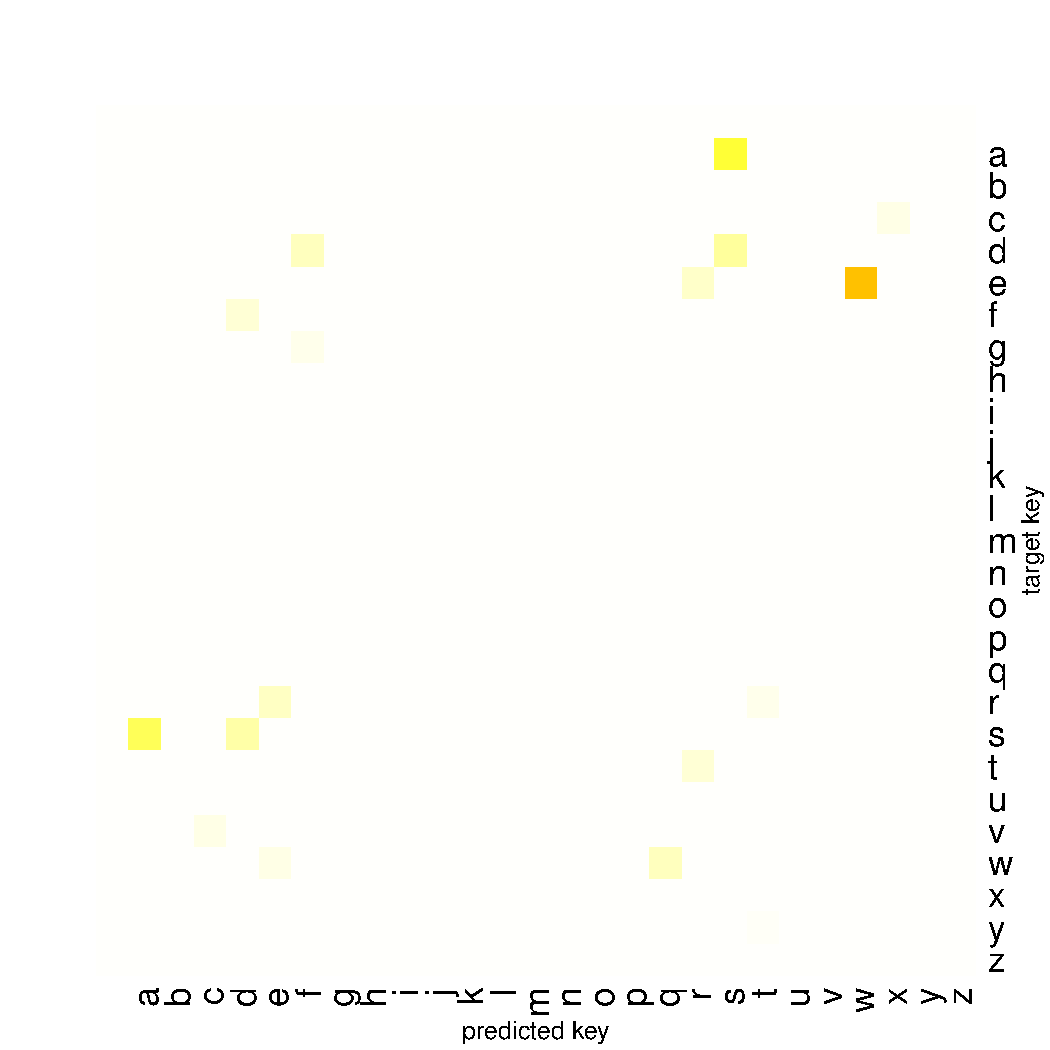
\includegraphics[width=0.49\columnwidth]{figures/sim-result-1-2.pdf}
%     \label{fig:error-key-posture}
%   }
%   \subfigure[Errors when using posture and key-adaptive model but not when using key-
%   adaptive model]{
%     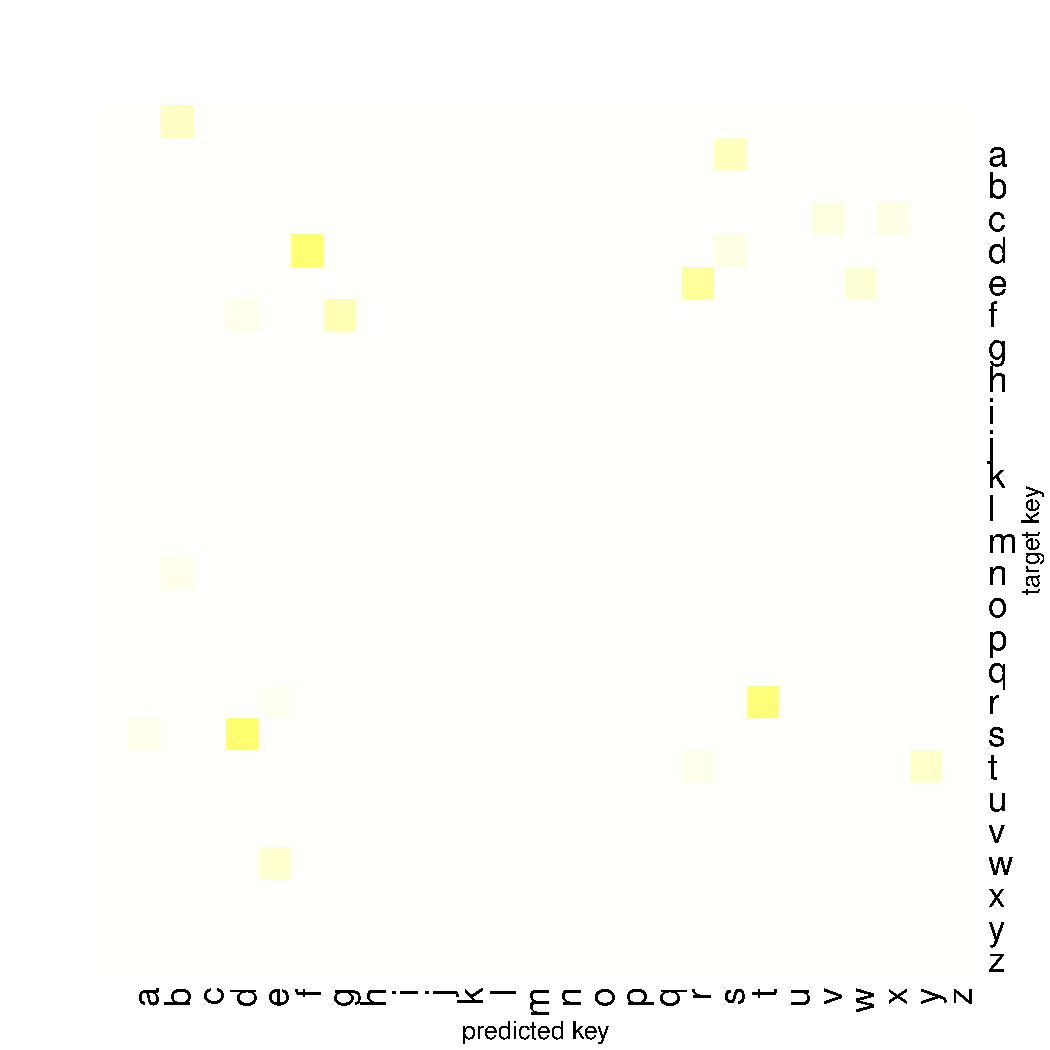
\includegraphics[width=0.49\columnwidth]{figures/sim-result-2-1.pdf}
%     \label{fig:error-posture-key}
%   }
%   \subfigure{
%     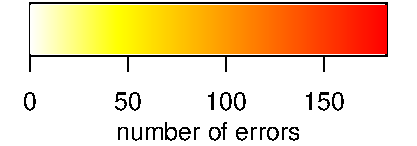
\includegraphics[width=0.3\columnwidth]{figures/sim-result-colorkey.pdf}
%   }
%   \caption{Confusion matrices for key estimation evaluation with different
%   spatial models as the highest order model. The row labels are the
%   target keys, and the column labels are the predicted keys.  The color of the cells
% represents the number of errors for a particular pair of confusion. The more red the color,
% the greater the number of errors.}
%   \label{fig:confusion-matrices}
% \end{figure*}

% The most number of corrections by using posture- and key-adaptive model is for
% the E and W pair. Figure~\ref{fig:e-w-ellipses} shows a closer look at the Gaussian distributions for the two keys for the different
% adaptive models. We can see the Gaussian distributions for key-adaptive model (black ellipses) shift slightly to the right. This causes the touch points on the boundary between W and
% E to be mis-classified as W. However, the ellipses based on the posture- and key-
% adaptive model for the two-thumb input shift to the left slightly, and this changes
% the classification of those boundary points to E correctly.

% \begin{figure}[tb]
%   \centering
%   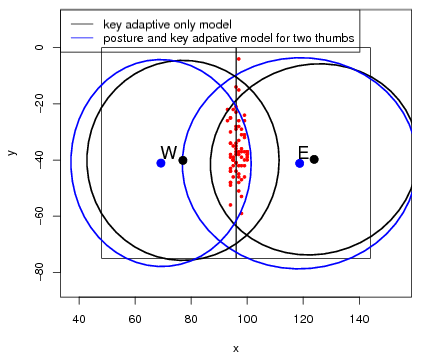
\includegraphics[width=1\columnwidth]{figures/key-posture-ellipse.png}
%   \caption{Each ellipse represents the 0.95 confidence ellipse of the Gaussian model built based on a set of touch points. Each black ellipse is based on the all touch points intended for either W or E. Each blue ellipse is based on touch points from two-thumb input only. The red points are the touch points intended for E but are mis-classified as W when using the key-adaptive model.
% }
%   \label{fig:e-w-ellipses}
% \end{figure}

\subsubsection{User Adaptation}
When computing the user- and key-adaptive model, for every touch point
we calculate the probability for each key given the underlying spatial model.
Then we use the $(x, y)$ coordinates of the touch point to update the Gaussian model for the most probable key. Updating the Gaussian model involves computing the running average of the $(x, y)$ offsets from the center of the key and the covariance matrices. The counter for the number of points used for a particular key Gaussian is maintained so that we
know when a particular Gaussian model is \textit{mature}. When there are not enough data points, the system backs-off to a lower level model.

We set the minimum number of points needed to build the
Gaussian model for a particular key and user pair to be 50.
Ideally we would want to set this number higher for better model reliability as
shown in Figure~\ref{fig:user-adapt}. However the current number is limited by
the amount of data available.  Only about half of the keys
have more than 50 data points for each user. The average number of data
points per key per individual is about 80. We chose 50 as a middle ground so
that there is room for individual adaptations for most of the keys. In a deployed system,
the data limitation will not be an issue. Alternatively, the system can use a user's data to
update the combined model. In this case the minimum
number required can be used to weigh the combined model with the personalized data.

\subsubsection{Posture, User, and Key Adaptation}
Tying everything together, the last row in Table~\ref{tab:off-device} shows the
error rate when the highest level model is posture-, user- and key-adaptive.
It reduces the error rate of the base model by 13.2\% ($(8.64 - 7.50) / 8.64$). The reduction is significant based on
the two-sample one-sided paired t-test (t(9) = 2.58, p = 0.015).

Figure~\ref{fig:partial-hierarchy} shows the backoff mechanism when there is insufficient data for the highest level model. The results based on our dataset in the "Comparison of Spatial Models" section suggest that we
can give higher priority to the user- and key-adaptive model when there is not enough data for
the highest level model. If there are still not enough data for that, we
can further backoff to the posture- and key-adaptive model.

\begin{figure}
 \centering
 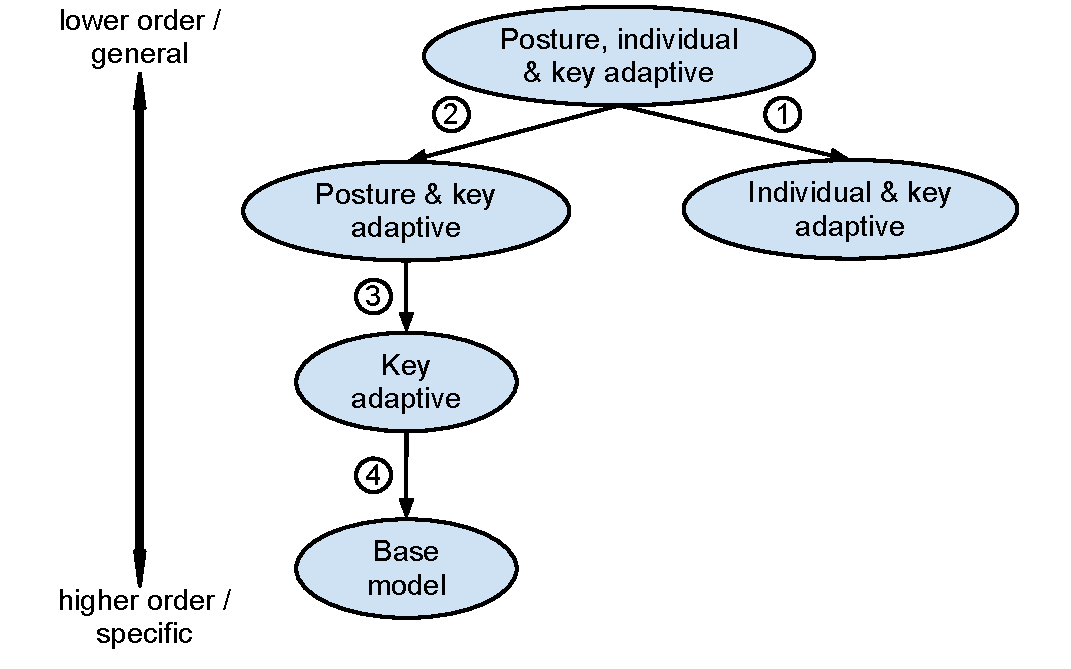
\includegraphics[width=0.9\columnwidth]{figures/partial-hierarchy.pdf}
 \caption{Partial hierarchical model implemented in our prototype. The numbers indicate the order of the
submodels to use during backoff.}
 \label{fig:partial-hierarchy}
\end{figure}
Note that because the dataset is a between-subjects study, we cannot study
the full effect of posture adaptation for each individual. We believe that there could be additional improvement, but further study is required to verify it.

\section{Discussion and Future Work}
We have shown the potential of posture, user, and key adaptation for
improving key estimation. An important limitation of our exploration thus far has been
the constraints of the dataset. To advance this line of work further we need more data than is typically available from lab experiments. Methods
such as real-use logging and game
playing~\cite{Rudchenko:2011} can be employed to gather a large body of
data. With this scale of data, the specific (sub)models, the
backoff procedure and sequence, and the parameters learned from the
data may change and be better optimized in the future.

In our proposed SBM, we switch from a more general to a more specific submodel
when a certain threshold of confidence is reached or enough data points are
collected. This is a binary decision, i.e., a submodel is either used or it is not.
Alternatively,
we can employ a mixture model that is a weighted average of
the general and the specific submodels (i.e., using soft decisions), with the
relative weight of the specific submodel increasing as confidence in it increases. We have started to experiment with this approach for user adaptation,
i.e., combining the individual data points with the combined model from the very beginning instead
of waiting until enough individual data points have been collected. Our preliminary studies have not shown a substantial difference, but our ongoing investigations may yield better results.
It is also worth noting that even though the mixture model approach may not
improve accuracy, it may provide a more gradual transition between submodels
and hence may provide a less disruptive user experience.

Once more data are collected to improve the SBM, more user studies can be run to validate how the system improves user typing
accuracy and speed. Of particular interest is how users
adapt their behavior to the SBM. For example, since posture adaptation
can tolerate different shifts left or right, might users respond by shifting their touch positions even further? Will users adopt the
tactic of choosing one posture and sticking to it in order to increase the system's
accuracy, and would it be desirable for them to do so? Might the sudden switch
by the system from one model to another disrupt interaction by making the input
method less predictable? All these are interesting HCI questions to be explored.

In this work, we combined the index-finger and one-thumb data together because
with the current touchscreen phones it is difficult to reliably
distinguish the two postures. But it may be possible to identify them by augmenting the
capacitive sensing with a range of frequencies that can help identify different kinds of
hand grips~\cite{Sato:2012}. Another possibility is to add a widget to the
keyboard that allows the user to optionally specify what posture they are
currently using. While this method can eliminate the posture
prediction error, it does so at the expense of overhead for the user. It would be interesting
to examine the trade-off between accuracy and time,
and users' preferences in this regard.

We have so far only considered the spatial model alone. More work is needed
to explore the interaction between spatial adaptation and language modeling.
As the language model can get fairly complex, our plan is to start with the
simplest one, e.g., one based on dictionary word frequencies, and then add
complexity step by step by, e.g., considering bigram frequencies, substitution,
elimination, and transposition errors.

Additional improvements in key estimation may be possible by extending the formulae in the ``Key Estimation Formulation'' section to consider a
sequence of touch points~\cite{Goodman:2002, Gunawardana:2010} instead of just one.
It would also be interesting to study how to use posture detection to guide
transposition error correction, because transposition errors are more likely to
occur when two hands are used to type.

\section{Conclusion}
We have introduced and evaluated a novel hierarchical adaptive spatial model for
touchscreen keyboards. Through comparative submodel analysis and evaluation of a prototype implementation, we have shown that both posture and user adaptation for a spatial model can improve key estimation accuracy. When posture, user, and key adaptations are combined, they
achieve the greatest improvement. For real-world
implementations, the
hierarchical structure gives a systematic way of backing-off to successively simpler models  when data is limited
or when there is insufficient confidence in higher level models.

We have also developed a new touchscreen input posture classification method
that achieves an accuracy of 86.4\% for classifying one-finger and two-thumb input. When
combined with the adaptive spatial model, the our analysis shows that the overall key detection increases significantly.

Our work also opens up many more interesting HCI questions in adaptive STK
that may not have been previously considered. We think that addressing these questions
will help improve the user experience with STK as touchscreen
devices become even more ubiquitous.

\section{Acknowledgements}
We want to thank our team members (names omitted for review) for their insightful
suggestions and help in  our data analysis and implementation of the prototype.
\balance
% If you want to use smaller typesetting for the reference list,
% uncomment the following line:
\small
\bibliographystyle{acm-sigchi}
\bibliography{chi2013}
\end{document}

